\documentclass{standalone}
\usepackage{pgfplots}
\pgfplotsset{compat=1.16}

\begin{document}
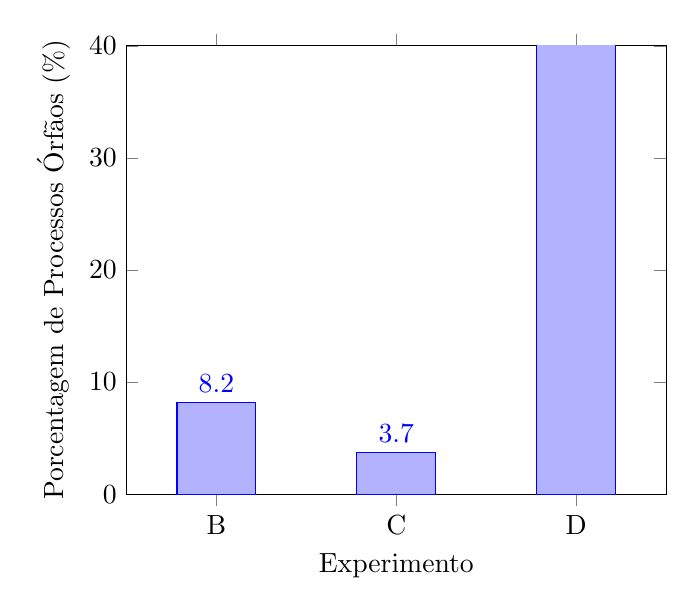
\begin{tikzpicture}
\begin{axis}[
    ybar,
    bar width=1cm,
    xlabel={Experimento},
    ylabel={Porcentagem de Processos Órfãos (\%)},
    symbolic x coords={B, C, D},
    xtick=data,
    ymin=0, ymax=40,
    nodes near coords,
    nodes near coords align={vertical},
    enlarge x limits=0.25,
    ]
\addplot coordinates {(B,8.2) (C,3.7) (D,42.7) };
\end{axis}
\end{tikzpicture}
\end{document}
